\documentclass[border=10pt]{standalone}

\usepackage{tikz}
\usepackage{tikzsymbols}
\usetikzlibrary{calc,patterns,shapes.geometric}

\def\centerarc[#1](#2)(#3:#4:#5){\draw[#1] ($(#2)+({#5*cos(#3)},{#5*sin(#3)})$) arc (#3:#4:#5);}

\begin{document}
	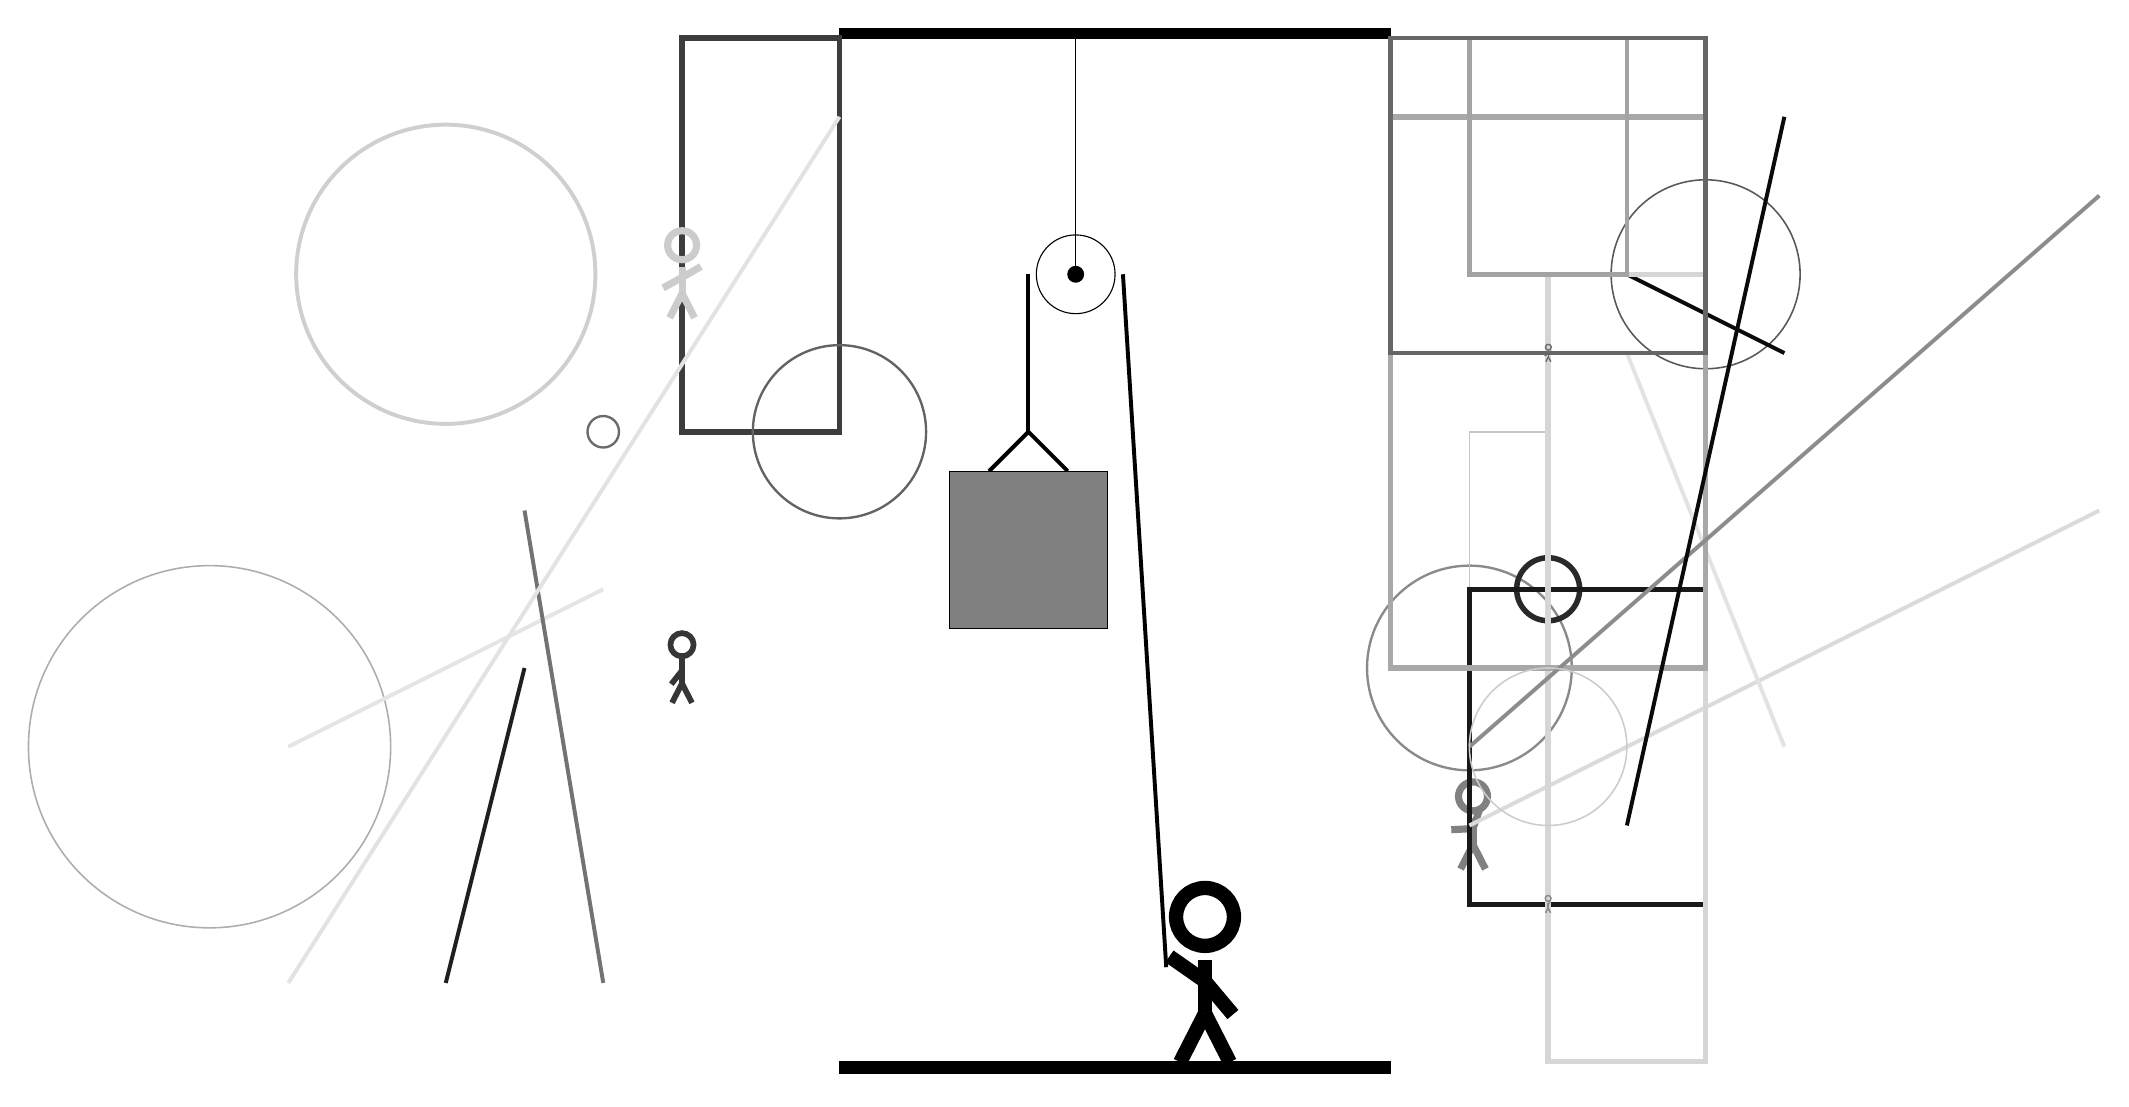
\begin{tikzpicture}
		%%%%% START %%%%%
		
		\draw[fill=black] (-2, 10) rectangle (5, 10.125);
		
		\draw (1, 7) circle (0.5);
		\draw[fill=black] (1, 7) circle (0.1);
		\draw (1, 10) -- (1, 7);
		
		\draw[line width=0.5mm] (-0.1, 4.5) -- (0.4, 5.0) -- (0.9, 4.5);
		\draw[fill=black!50] (-0.6, 4.5) rectangle (1.4, 2.5);
		
		\draw[line width=0.5mm] (0.4, 7) -- (0.4, 5.0);
		\centerarc[line width=0.5mm](1, 7)(0:180:0.6);
		\draw[line width=0.5mm](1.6, 7) -- (2.15, -1.8);
		
		\draw [line width=0.2mm, color=black!65](9, 7) circle (1.2);
		
		\draw [line width=0.3mm, color=black!46](6, 2) circle (1.3);
		\draw [line width=0.7mm, color=black!84](7, 3) circle (0.4);
		\node[line width=0.4mm, color=black!50] at (6, 0) {\Strichmaxerl[5][3][71]};
		\draw[line width=0.7mm, color=black!76] (-2, 5) rectangle (-4, 10);
		
		\draw[line width=0.2mm, color=black!22] (7, 5) rectangle (6, 2);
		
		\draw [line width=0.2mm, color=black!32](-10, 1) circle (2.3);
		\draw[line width=0.6mm, color=black!90] (6, 3) rectangle (9, -1);
		\draw[line width=0.5mm, color=black!14](6, 0) -- (14, 4);
		\draw[line width=0.5mm, color=black!96](10, 6) -- (8, 7);
		\draw [line width=0.5mm, color=black!19](-7, 7) circle (1.9);
		\node[line width=0.2mm, color=black!79] at (-4, 2) {\Strichmaxerl[4][52][90]};
		\draw[line width=0.7mm, color=black!16] (7, 7) rectangle (9, -3);
		\draw [line width=0.3mm, color=black!61](-2, 5) circle (1.1);
		\node[line width=0.7mm, color=black!20] at (-4, 7) {\Strichmaxerl[5][29][30]};
		\draw [line width=0.3mm, color=black!58](-5, 5) circle (0.2);
		
		\draw[line width=0.5mm, color=black!88](-6, 2) -- (-7, -2);
		\draw[line width=0.5mm, color=black!10](-5, 3) -- (-9, 1);
		\draw[line width=0.5mm, color=black!11](10, 1) -- (8, 6);
		\draw[line width=0.7mm, color=black!34] (5, 2) rectangle (9, 9);
		\node[line width=0.5mm, color=black!46] at (7, -1) {\Strichmaxerl[1][88][63]};
		
		\draw[line width=0.5mm, color=black!55](-5, -2) -- (-6, 4);
		\draw[line width=0.6mm, color=black!36] (6, 7) rectangle (8, 10);
		\node[line width=0.7mm, color=black!59] at (7, 6) {\Strichmaxerl[1][31][41]};
		\draw[line width=0.5mm, color=black!45](6, 1) -- (14, 8);
		\draw[line width=0.5mm, color=black!96](8, 0) -- (10, 9);
		\draw [line width=0.2mm, color=black!20](7, 1) circle (1.0);
		\draw[line width=0.5mm, color=black!11](-2, 9) -- (-9, -2);
		\draw[line width=0.6mm, color=black!60] (5, 6) rectangle (9, 10);
		
		\node at (2.6, -1.9) {\Strichmaxerl[10][-35][-50]};
		
		\draw[fill=black] (-2, -3) rectangle (5, -3.15);
		
		%%%%% END %%%%%
	\end{tikzpicture}
\end{document}